%!TEX TS-program = xelatex
\documentclass[12pt, a4paper]{article}  

\usepackage{etex} % расширение классического tex в частности позволяет подгружать гораздо больше пакетов, чем мы и займёмся далее

%%%%%%%%%% Математика %%%%%%%%%%
\usepackage{amsmath,amsfonts,amssymb,amsthm,mathtools} 
%\mathtoolsset{showonlyrefs=true}  % Показывать номера только у тех формул, на которые есть \eqref{} в тексте.
%\usepackage{leqno} % Нумерация формул слева


%%%%%%%%%%%%%%%%%%%%%%%% Шрифты %%%%%%%%%%%%%%%%%%%%%%%%%%%%%%%%%
\usepackage{fontspec}         % пакет для подгрузки шрифтов
\setmainfont{Arial}   % задаёт основной шрифт документа

\defaultfontfeatures{Mapping=tex-text}

% why do we need \newfontfamily:
% http://tex.stackexchange.com/questions/91507/
\newfontfamily{\cyrillicfonttt}{Arial}
\newfontfamily{\cyrillicfont}{Arial}
\newfontfamily{\cyrillicfontsf}{Arial}

\usepackage{unicode-math}     % пакет для установки математического шрифта
\setmathfont{Asana Math}      % шрифт для математики
% \setmathfont[math-style=ISO]{Asana Math}
% Можно делать смену начертания с помощью разных стилей

% Конкретный символ из конкретного шрифта
% \setmathfont[range=\int]{Neo Euler}

\usepackage{polyglossia}      % Пакет, который позволяет подгружать русские буквы
\setdefaultlanguage{russian}  % Основной язык документа
\setotherlanguage{english}    % Второстепенный язык документа


%%%%%%%%%% Работа с картинками %%%%%%%%%
\usepackage{graphicx}                  % Для вставки рисунков
\usepackage{graphics}
\graphicspath{{images/}{pictures/}}    % можно указать папки с картинками
\usepackage{wrapfig}                   % Обтекание рисунков и таблиц текстом
\usepackage{color}

%%%%%%%%%% Работа с таблицами %%%%%%%%%%
\usepackage{tabularx}            % новые типы колонок
\usepackage{tabulary}            % и ещё новые типы колонок
\usepackage{array}               % Дополнительная работа с таблицами
\usepackage{longtable}           % Длинные таблицы
\usepackage{multirow}            % Слияние строк в таблице
\usepackage{float}               % возможность позиционировать объекты в нужном месте
\usepackage{booktabs}            % таблицы как в книгах!
\renewcommand{\arraystretch}{1.3} % больше расстояние между строками

% Заповеди из документации к booktabs:
% 1. Будь проще! Глазам должно быть комфортно
% 2. Не используйте вертикальные линни
% 3. Не используйте двойные линии. Как правило, достаточно трёх горизонтальных линий
% 4. Единицы измерения - в шапку таблицы
% 5. Не сокращайте .1 вместо 0.1
% 6. Повторяющееся значение повторяйте, а не говорите "то же"
% 7. Есть сомнения? Выравнивай по левому краю!





%%%%%%%%%% Графика и рисование %%%%%%%%%%
\usepackage{tikz, pgfplots}  % язык для рисования графики из latex'a
\usepackage{amscd}                  %Пакеты для рисования
\usepackage[matrix,arrow,curve]{xy} %комунитативных диаграмм


%%%%%%%%%% Теоремы %%%%%%%%%%
\theoremstyle{plain}              % Это стиль по умолчанию.  Есть другие стили. 
\newtheorem{theorem}{Теорема}[section]
\newtheorem{result}{Следствие}[theorem]
% счётчик подчиняется теоремному, нумерация идёт по главам согласованно между собой

\theoremstyle{definition}         % убирает курсив и что-то еще наверное делает ;)
\newtheorem*{defin}{Определение}  % нумерация не идёт вообще

\newtheorem{fignia}{Какая-то фигня}




%%%%%%%%%% Свои команды %%%%%%%%%%
\usepackage{etoolbox}    % логические операторы для своих макросов


% Все свои команды лучше всего определять не по ходу текста, как это сделано в этом документе, а в преамбуле!




% Пакет, который ставит в каждом первом абзаце главы красную строку
% Просто, чтобы эта pdf-ка нормально смотрелась :)
%\usepackage{indentfirst}
%\setkeys{russian}{babelshorthands=true}
\DeclareMathOperator{\Var}{Var}
\DeclareMathOperator{\Cov}{Cov}
\DeclareMathOperator{\Corr}{Corr}

\title{Домашнее задание 3. \\ Упражнение 1}
\author{Решетникова Дарья}
\date{\today}

\begin{document}

\maketitle



% так как в пункте данного задания про картинки требуется, чтобы выводился номер секции, все подпункты представлены отдельными секциями, хотя мне больше нравится, когда подсекциями..
\section{}

Например, $\Var$ это дисперсия.\\
А это: $\Cov$ -- ковариация.\\
Ну и, наконец, $\Corr$ -- корреляция. \\

\section{}
\newcommand{\s}{$\sigma$}

А вот и \s-алгебра подъехала. \\
\newcommand{\sa}{$\sigma$-алгебра}
Ну, или можно так \sa. 

\section{}
\newcommand{\xdot}{$x_1 \ldots x_n$}
Так мы получим \xdot \\
\newcommand{\com}[2]{x_{#1} \ldots x_{#2}}
А можем получить и так $\com{1}{n}$, а еще это $\com{a}{z}$, и это, $\com{1}{6}$, ну и это $\com{(a,b)}{(c,d)}$

\section{}
\renewcommand{\labelitemi}{${\color{blue}\bullet}$}
\begin{itemize}
	\item Пункт первый
	\item Пункт второй
	\item Пункт третий
\end{itemize}

\section{}
\newcommand{\llim}{\lim\limits_{x \to 0} \frac{\sin x}{x}}
А вот и $\llim$.
\[\llim\]

\section{}

\renewcommand{\theequation}{Eq. (\arabic{equation})}
\setcounter{equation}{0} 

\begin{equation}
	\lim\limits_{x \to 0} \frac{\sin x}{x}=1
\end{equation}

\begin{equation}
\llim =1
\end{equation}

\section{}

\renewcommand{\thefigure}{\thesection:\arabic{figure}}
\setcounter{figure}{0} 

\begin{figure}[H]
	\begin{center}
		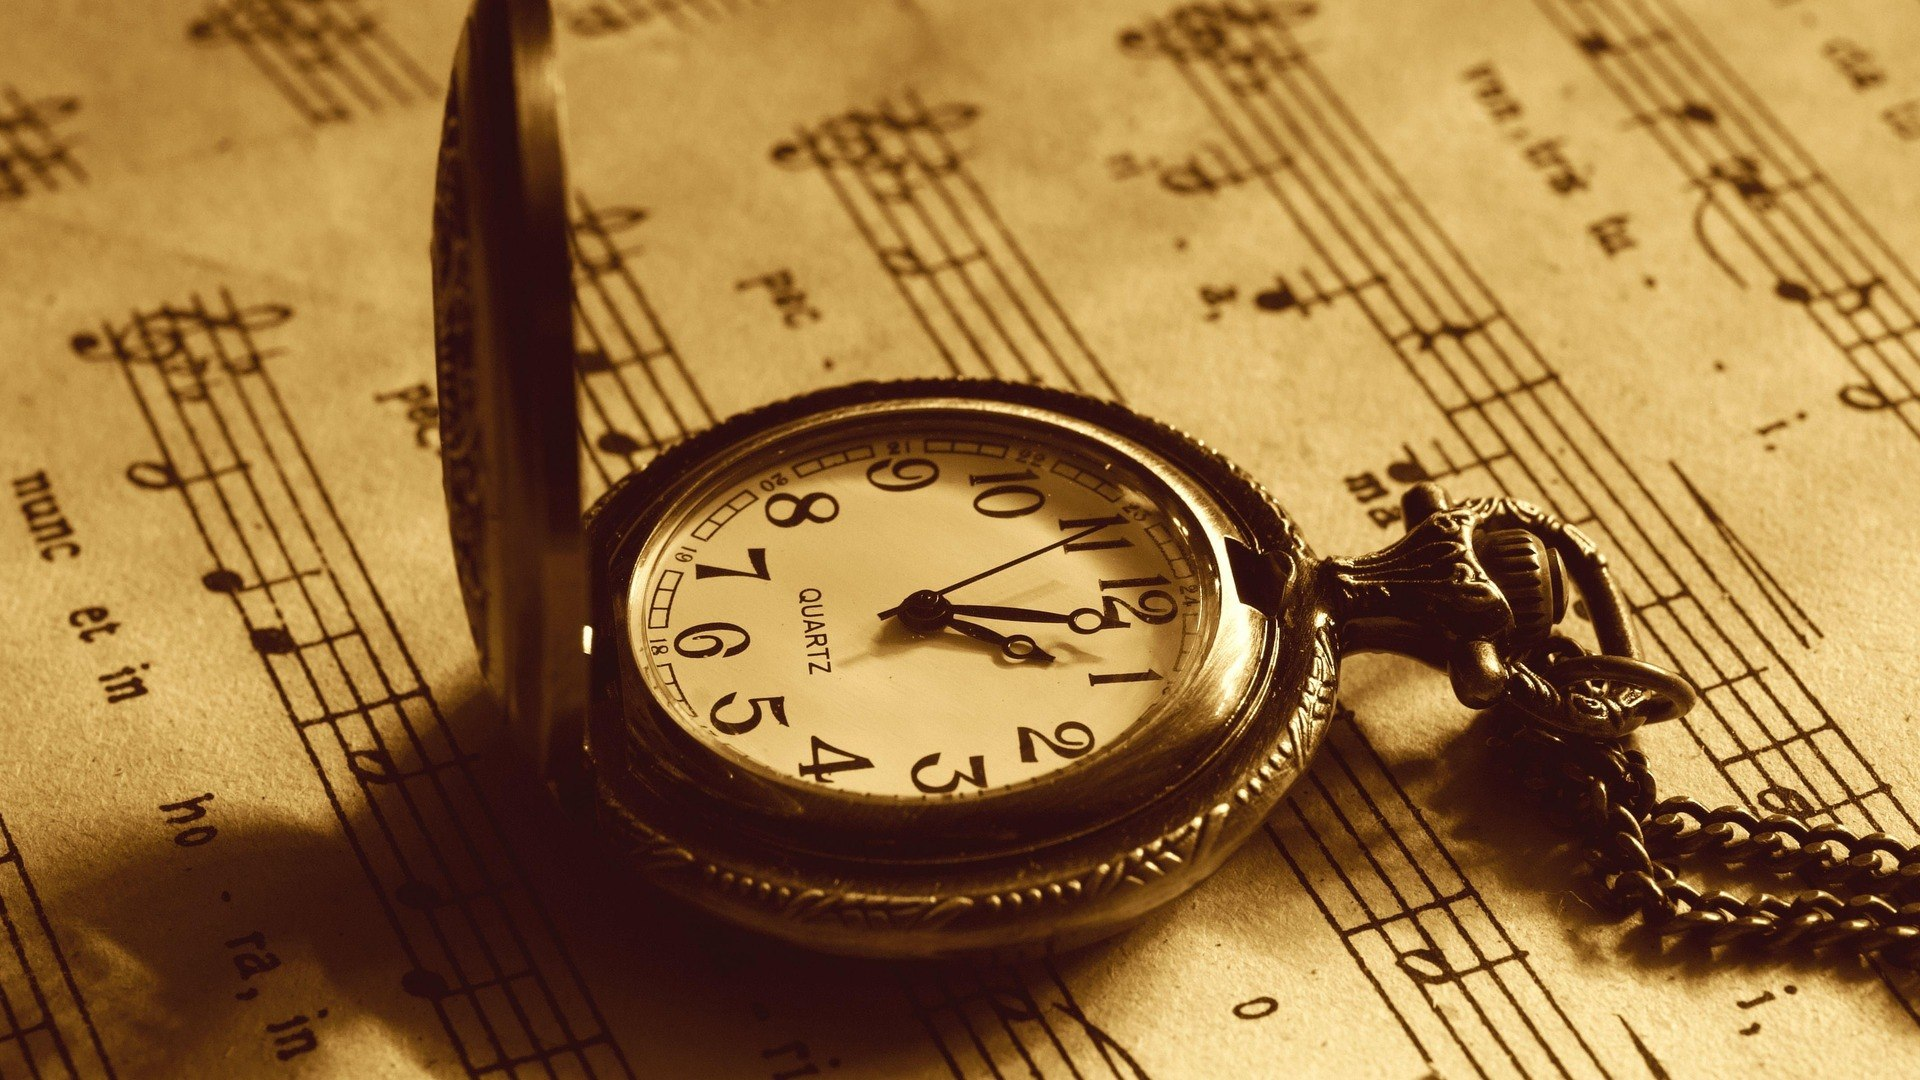
\includegraphics[scale=0.2]{pic.jpg} 
	\end{center}
	\caption{Самый дорогой ресурс человечества}
\end{figure}

\section{}

\newenvironment{rottext}{
	\newcommand{\rt}[2]{\rotatebox{180}{##1} \reflectbox{##2}}
}{}
\begin{rottext}
	\rt{Здесь должен быть какой то текст.}{Но я не придумала какой.}
\end{rottext}


\end{document}
